


\chapter{nginx}

Vamos a comenzar enviando el directorio con \verb|tar|, de forma simple. Comenzamos creando un directorio con un archivo como se ve en \eqref{enviar_1}.

\begin{figure}[h!]
\begin{center}
\caption{Creación de directorio con un archivo en m1 y contenido de este archivo.}
\label{enviar_1}
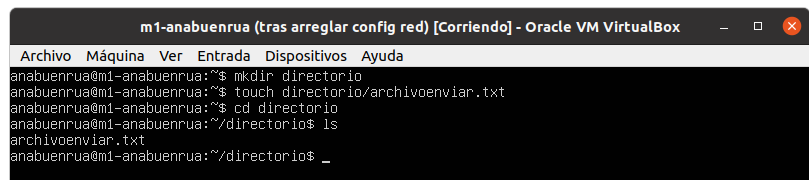
\includegraphics[scale=0.5]{enviar_1}
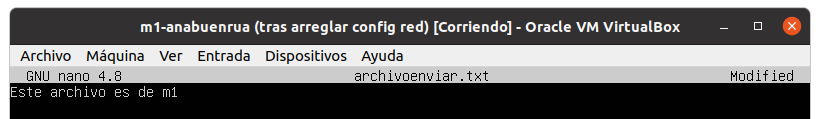
\includegraphics[scale=0.5]{enviar_2}
\end{center}
\end{figure}

Y mandamos el directorio comprimido con tar \eqref{enviar_3}. Como ya configuramos el acceso por ssh sin contraseña no nos la pide.

\begin{figure}[h!]
\begin{center}
\caption{Envío del archivo comprimido con tar}
\label{enviar_3}
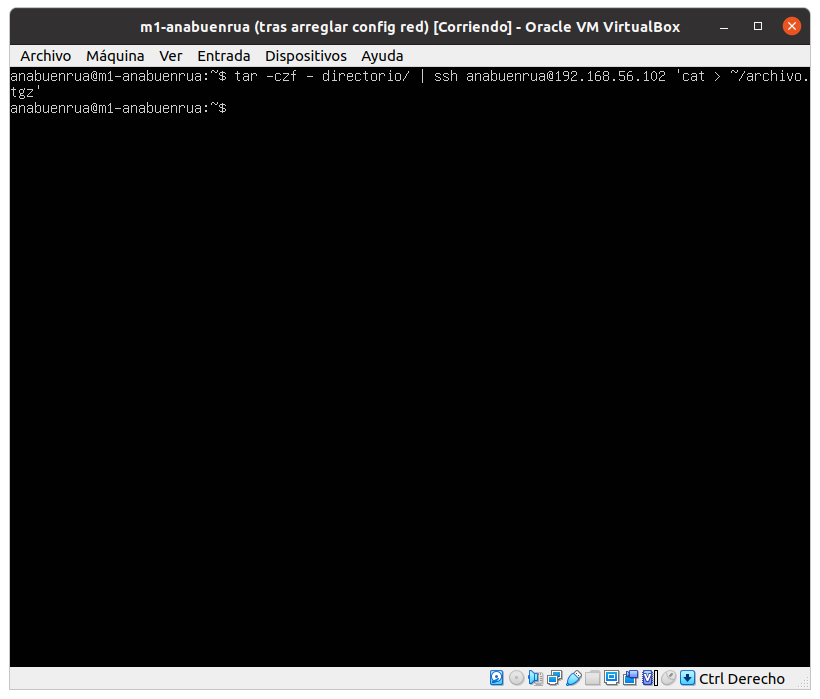
\includegraphics[scale=0.5]{enviar_3}
\end{center}
\end{figure}

Finalmente descomprimimos y comprobamos que se ha mandado correctamente \eqref{enviar_4}.

\begin{figure}[h!]
\begin{center}
\caption{Descompresión y comprobación del envío correcto del archivo.}
\label{enviar_4}
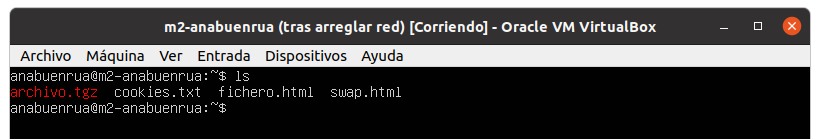
\includegraphics[scale=0.5]{enviar_4}
\end{center}
\end{figure}

\section{Envío mediante tar y scp}

Ahora vamos a enviarlo mediante tar y scp. Para ello creamos el tar y lo mandamos mediante scp como se ve en \eqref{enviar_6}

\begin{figure}[h!]
\begin{center}
\caption{Compresión con tar y envío mediante scp}
\label{enviar_6}
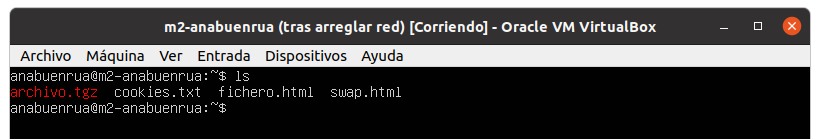
\includegraphics[scale=0.5]{enviar_4}
\end{center}
\end{figure}

Comprobamos en \eqref{enviar_7} que en la máquina 2 se encuentra directorio2.

\begin{figure}[h!]
\begin{center}
\caption{Comprobación de la llegada de directorio2 a m2}
\label{enviar_7}
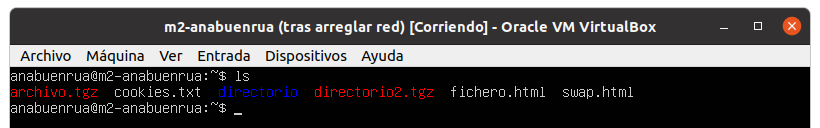
\includegraphics[scale=0.5]{enviar_7}
\end{center}
\end{figure}

\section{Comandos avanzados}

Vamos a enviar el directorio esta vez usando scp y algunas de sus opciones.

Comenzamos son \verb|-r|, que copia recursivamente directorios enteros, y \verb|-v| nos da información de la copia y de ssh. Como vemos en \eqref{enviar_8} muestra mucha información.

\begin{figure}[h!]
\begin{center}
\caption{Uso de scp con comandos avanzados}
\label{enviar_8}
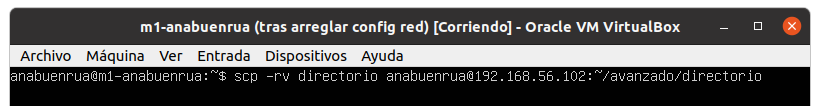
\includegraphics[scale=0.5]{enviar_8}
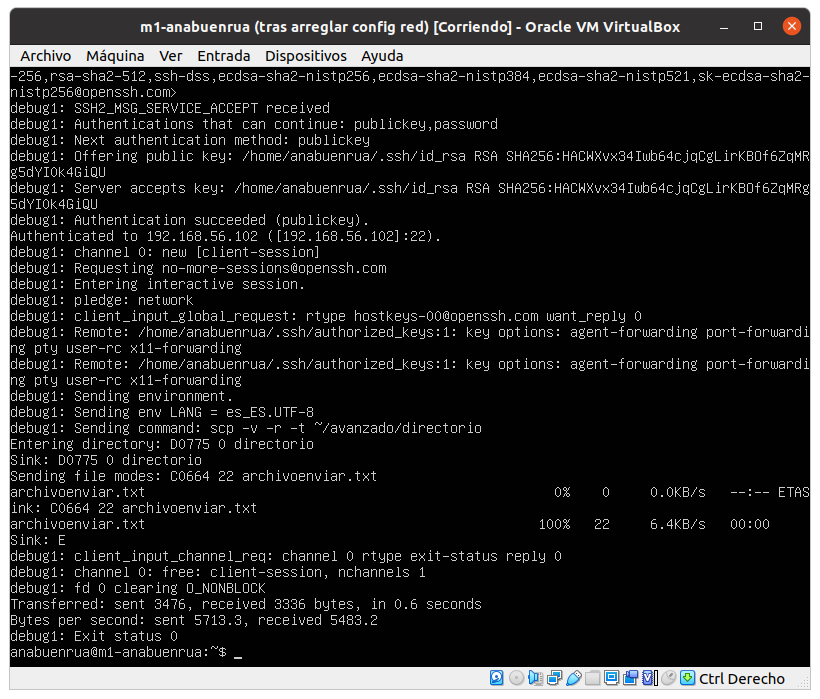
\includegraphics[scale=0.5]{enviar_9}
\end{center}
\end{figure}

También podemos usar la opción \verb|-q| que desactiva que se muestren mensajes por si se mandan muchos archivos \eqref{enviar_11}

\begin{figure}[h!]
\begin{center}
\caption{Uso de scp con comandos avanzados}
\label{enviar_11}
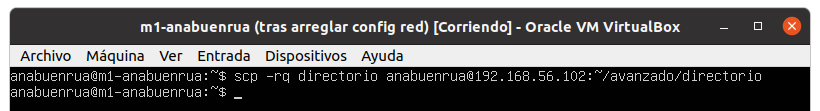
\includegraphics[scale=0.5]{enviar_11}
\end{center}
\end{figure}

Finalmente, con \verb|-P| podemos indicar el puerto. Por ejemplo de m2 a m1 como se muestra en \eqref{enviar_13}

\begin{figure}[h!]
\begin{center}
\caption{Uso de scp con comandos avanzados}
\label{enviar_13}
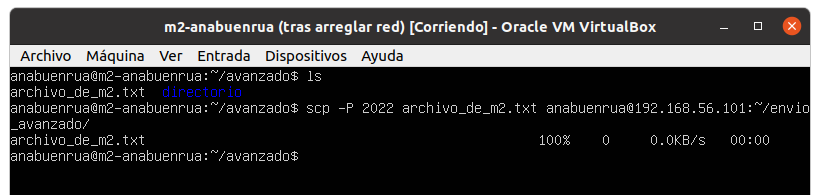
\includegraphics[scale=0.5]{enviar_13}
\end{center}
\end{figure}


\chapter{Utilizando Rsync}

Rsync ya está instalado en ambas máquinas, comprobamos su versión en \eqref{rsync_1}

\begin{figure}[h!]
\begin{center}
\caption{Comprobación de la versión de Rsync.}
\label{rsync_1}
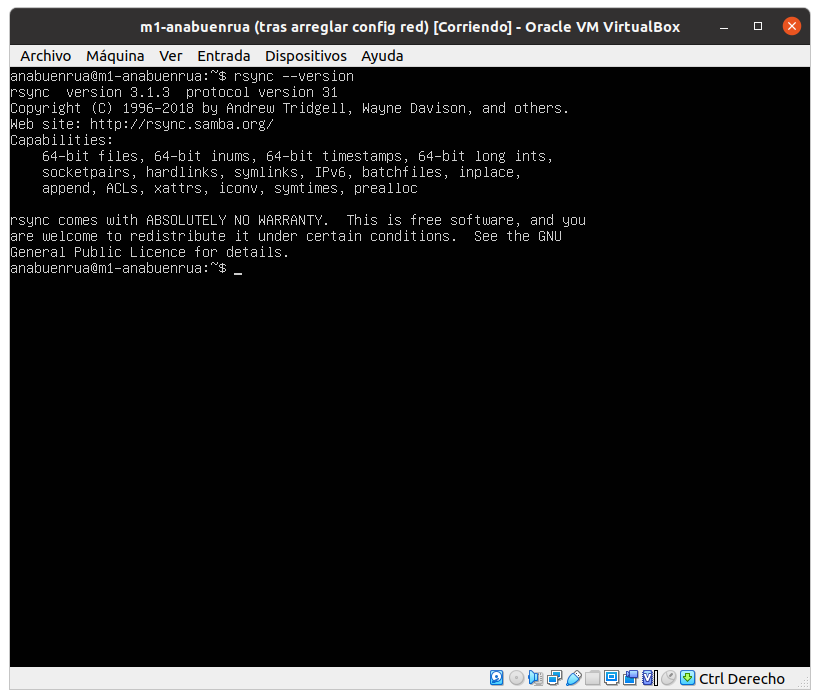
\includegraphics[scale=0.5]{rsync_1}
\end{center}
\end{figure}

Con chown cambiamos el propietario de la carpeta \verb|/var/www/| ejecutando el comando \eqref{rsync_2}

\begin{figure}[h!]
\begin{center}
\caption{Cambiamos el propietario de la carpeta /var/www/}
\label{rsync_2}
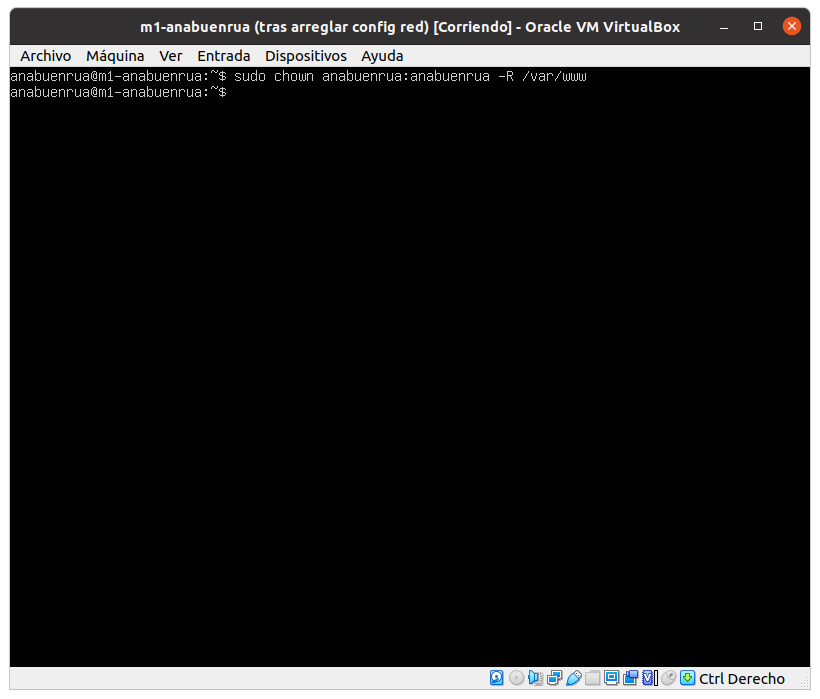
\includegraphics[scale=0.5]{rsync_2}
\end{center}
\end{figure}

Y ejecutamos rsync en m1, para copiar los archivos a m2, como se muestra en \eqref{rsync_4}:

\begin{figure}[h!]
\begin{center}
\caption{Sincronización de la carpeta /var/www/ de m1 a m2}
\label{rsync_4}
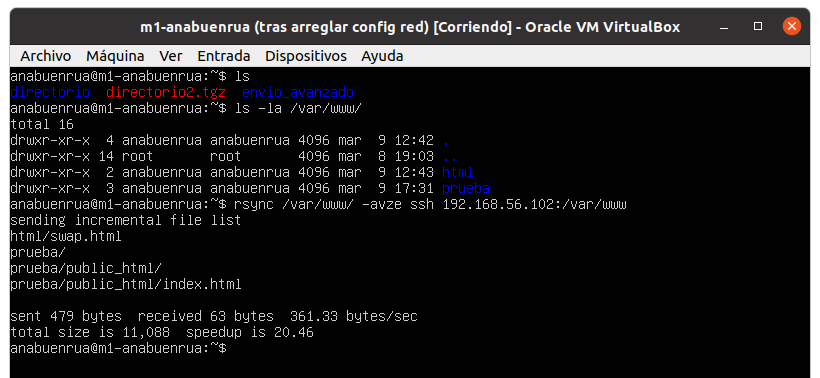
\includegraphics[scale=0.5]{rsync_4}
\end{center}
\end{figure}

Las opciones usadas son \verb|-a|, que indica recursividad (archive), \verb|-e| especifica el shell remoto que se va a utilizar, \verb|-v| es verbose, para dar más información y \verb|-z| para comprimir los archivos durante la trasnferencia.

\section{Opciones avanzadas}

Como opciones avanzadas vamos a usar \verb|--stats|, que nos muestra estadísticas, \verb|--exclude|, para excluir carpetas o directorios, \verb|--delete|, para borrar en la máquina destino los ficheros borrados de la máquina origen y \verb|--dry-run|, que permite a rsync hacer un clonado de prueba, de forma que podemos ver lo que se va a clonar pero sin llegar a efectuarse la copia.

Comenzamos creando un directorio de prueba a clonar desde m1 a m2 \eqref{rsync_a1}.

\begin{figure}[h!]
\begin{center}
\caption{Creamos directorio de prueba para clonar usando rsync.}
\label{rsync_a1}
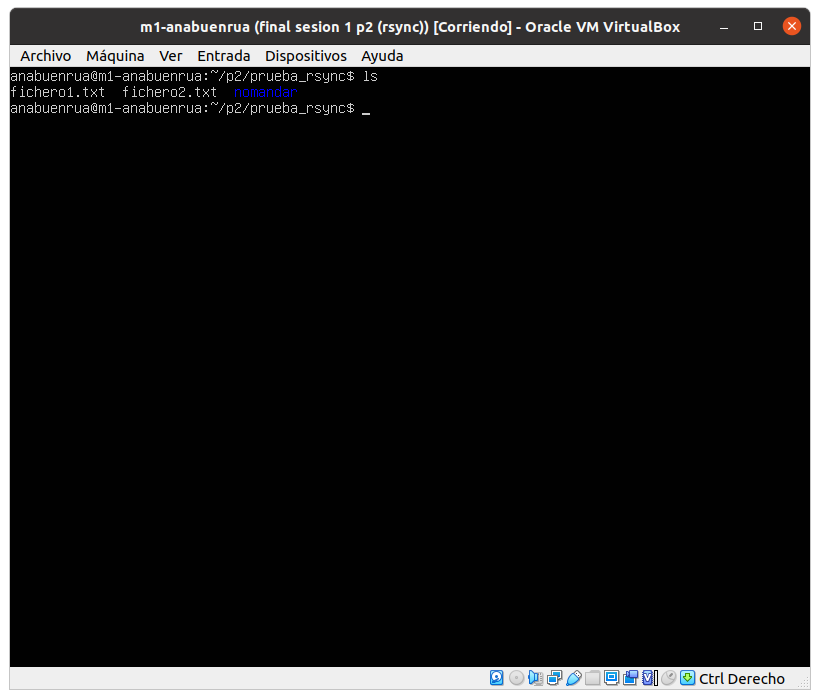
\includegraphics[scale=0.5]{rsync_a1}
\end{center}
\end{figure}

Comenzamos realizando una prueba de lo que sería la copia con \verb|--dry-run|, como mostramos en \eqref{rsync_a2}.

\begin{figure}[h!]
\begin{center}
\caption{Ejecución de rsync don --dry-run}
\label{rsync_a2}
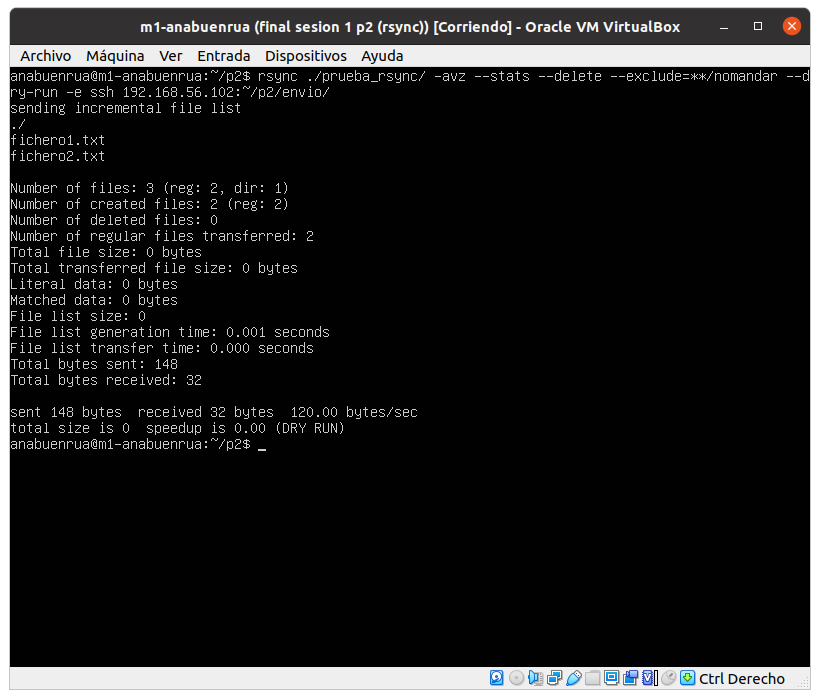
\includegraphics[scale=0.5]{rsync_a2}
\end{center}
\end{figure}

Así, comprobamos que en efecto se va a mandar lo que queremos, pero todavía no hemos clonado nada, como podemos comprobar en la máquina m2, se puede ver en \eqref{rsync_a3}

\begin{figure}[h!]
\begin{center}
\caption{Estado de m2 tras la ejecución de rsync con --dry-run}
\label{rsync_a3}
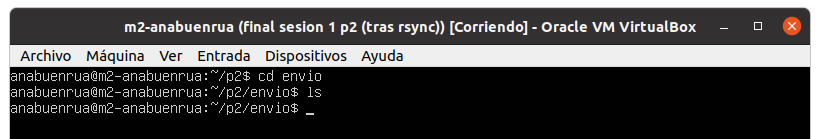
\includegraphics[scale=0.5]{rsync_a3}
\end{center}
\end{figure}

Ahora sí, procedemos a realizar el envío quitando la opción \verb|--dry-run|, en \eqref{rsync_a4}, y comprobamos que se ha copiado con éxito en \eqref{rsync_a5}

\begin{figure}[h!]
\begin{center}
\caption{Ejecución de rsync con opciones avanzadas.}
\label{rsync_a4}
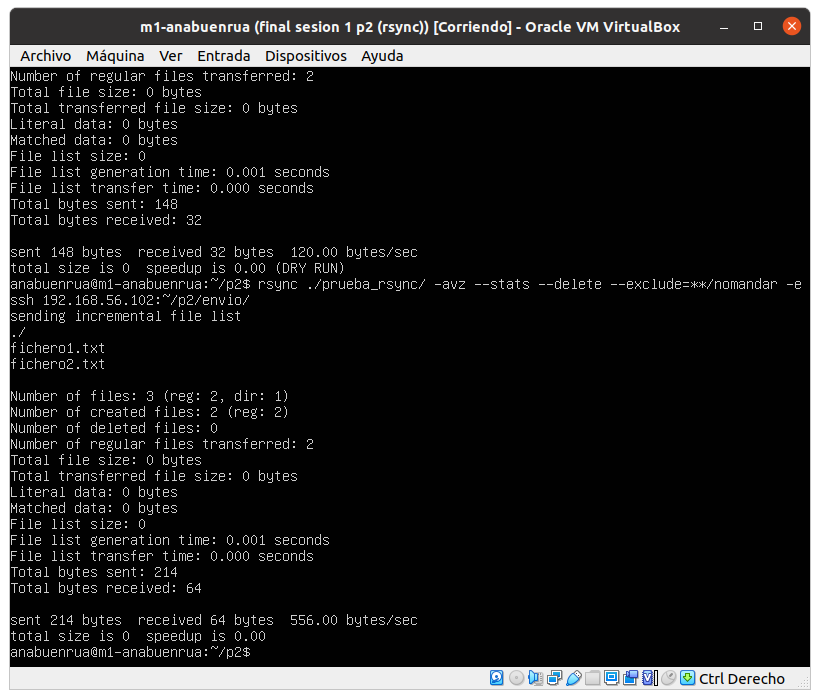
\includegraphics[scale=0.5]{rsync_a4}
\end{center}
\end{figure}

\begin{figure}[h!]
\begin{center}
\caption{Comprobando la copia correcta de los ficheros en m2.}
\label{rsync_a5}
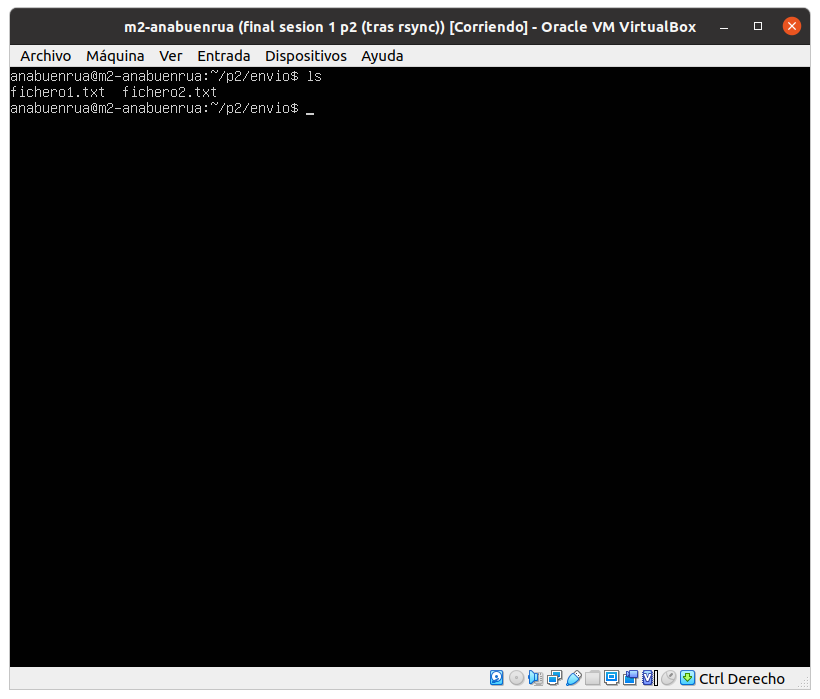
\includegraphics[scale=0.5]{rsync_a5}
\end{center}
\end{figure}

Es claro que el argumento \verb|--exclude| ha evitado que se copie el directorio \verb|nomandar|.

Finalmente, probamos a eliminar el fichero \verb|fichero1.txt| y repetir el clonado, comprobando así que la opción \verb|--delete| lo elimina en m2 también, como se ve en \eqref{rsync_a6}

\begin{figure}[h!]
\begin{center}
\caption{Ejecución de rsync tras borrar fichero1 en m1 y el resultado en m2}
\label{rsync_a6}
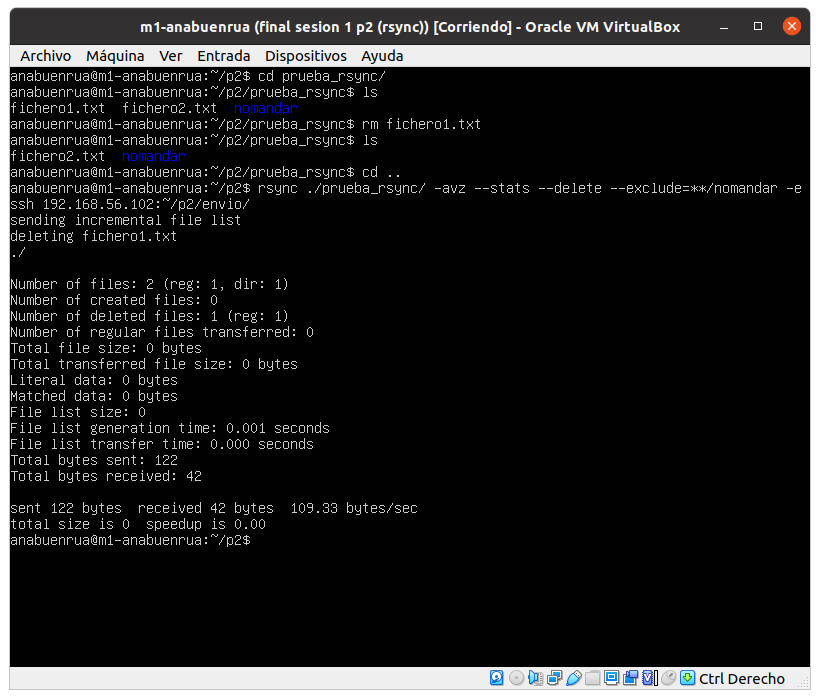
\includegraphics[scale=0.5]{rsync_a6}
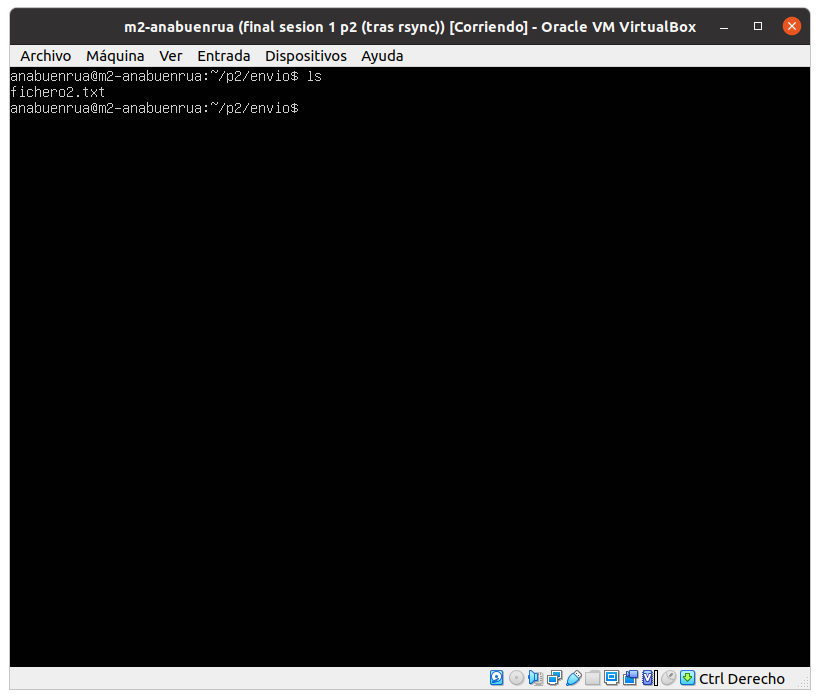
\includegraphics[scale=0.5]{rsync_a7}
\end{center}
\end{figure}

\chapter{Acceso mediante ssh sin contraseña}

El acceso por ssh sin introducir la contraseña manualmente ya se configuró en la práctica anterior.

Para ello, generamos en cada máquina una clave pública y privada, con \verb|ssh-keygen|, como se muestra en \eqref{ssh_1}.

\begin{figure}[h!]
\begin{center}
\caption{Generación de claves con ssh-keygen}
\label{ssh_1}
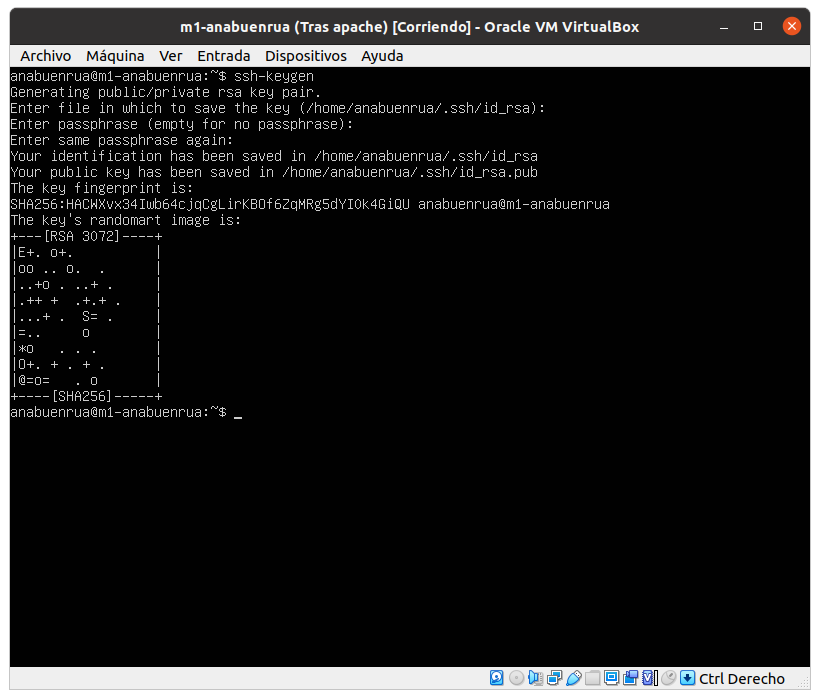
\includegraphics[scale=0.5]{ssh_1}
\end{center}
\end{figure}

Después compartimos las claves públicas de una máquina a otra con 

\verb|ssh-copy-id -p 2022 anabuenrua@192.168.56.101| (de m2 a m1) y

\verb|ssh-copy-id anabuenrua@192.168.56.102| (de m1 a m2). El caso de m2 a m1 puede verse en \eqref{ssh_2}

\begin{figure}[h!]
\begin{center}
\caption{Envío de claves públicas mediante ssh-sopy-id}
\label{ssh_2}
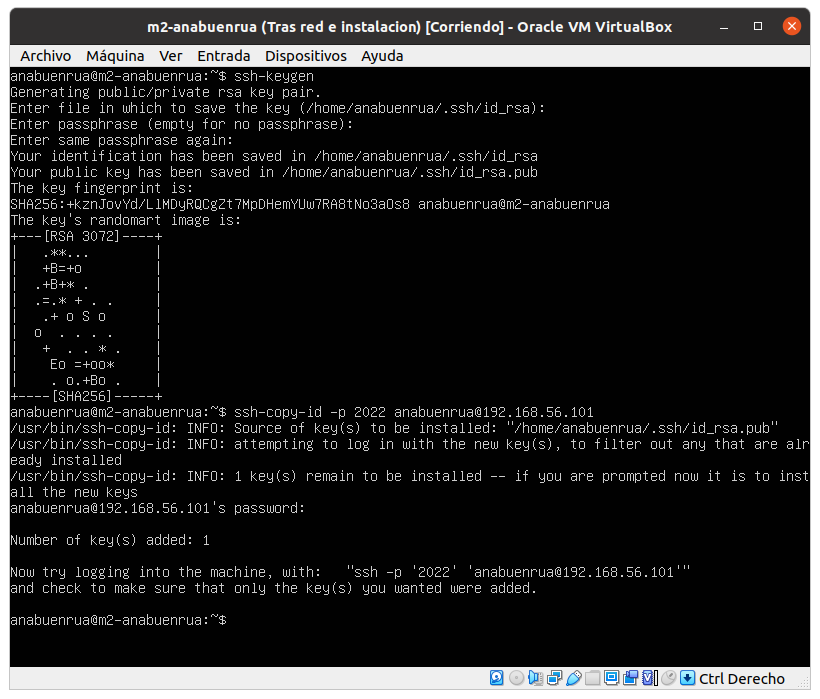
\includegraphics[scale=0.5]{ssh_2}
\end{center}
\end{figure}

\section{Opciones avanzadas}

Cuando se realizó, se dejaron todas las opciones por defecto, pero se pueden usar algunos argumentos para modificar el comportamiento:

\begin{itemize}
\item \verb|-t|: Especifica el tipo de clave que se va a generar, por ejemplo rsa.
\item \verb|-b|: Indica el número de bits en la clave, por defecto es 2048.
\item \verb|-f|: Especifica el archivo de la clave.
\item \verb|-l|: No se usa al generar las claves, si no que se usa para ver el fingerprint de una clave pública.
\item \verb|-v|: Verbose.
\end{itemize}

Ejemplos de uso de estos argumentos son \verb|ssh-keygen -t rsa -b 4096| o \eqref{ssh_3}.

\begin{figure}[h!]
\begin{center}
\caption{Opciones avanzadas de ssh-keygen}
\label{ssh_3}
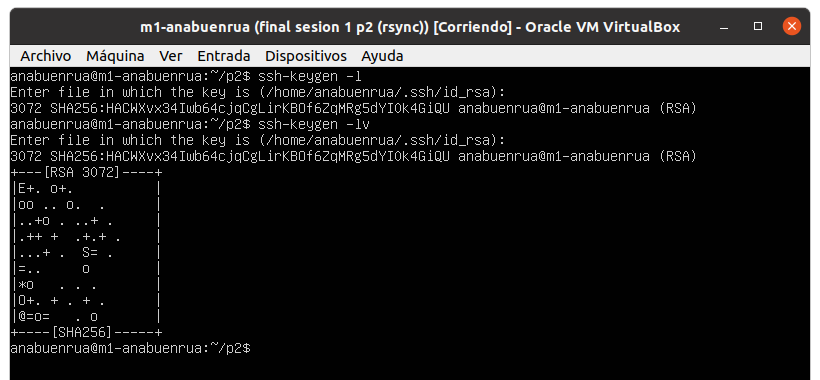
\includegraphics[scale=0.5]{ssh_3}
\end{center}
\end{figure}

Si al generar la clave no usamos la ruta por defecto, para mandarla con \verb|ssh-copy-id| debemos especificar la ruta de la clave pública con \verb|-i|, al igual que al acceder se especifica la de la clave privada con \verb|-i| en \verb|ssh|.

\section{Copia de clave manual}

Comenzamos en m2, accediendo a \verb|~/.ssh/authorized_keys|, donde está escrita la clave pública de \verb|m1|. Editamos este fichero con nano borrando su contenido y comprobamos que ahora para acceder a m2 desde m1 nos pide contraseña, \eqref{ssh_5}

\begin{figure}[h!]
\begin{center}
\caption{Comprobación de que nos requiere contraseña para conectar mediante ssh tras borrar la clave previamente guardada.}
\label{ssh_5}
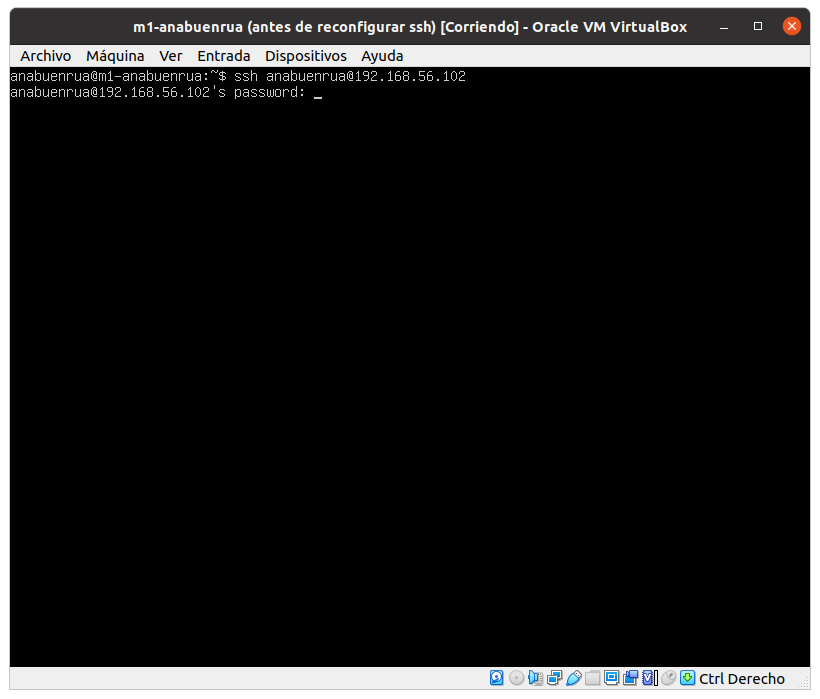
\includegraphics[scale=0.5]{ssh_5}
\end{center}
\end{figure}

Para volver a tener acceso sin contraseña, vamos a mandar nuestra clave pública a m2. Para ello copiamos la clave pública que se encuentra en \verb|~/.ssh/id_rsa.pub| de m1 mediante \verb|scp| en el archivo \verb|~/.ssh/authorized_keys| de m2, como vemos en \eqref{ssh_6}.

\begin{figure}[h!]
\begin{center}
\caption{Visualización y envío de la clave pública mediante scp y comprobación en la máquina m2 de que se ha realizado correctamente.}
\label{ssh_6}
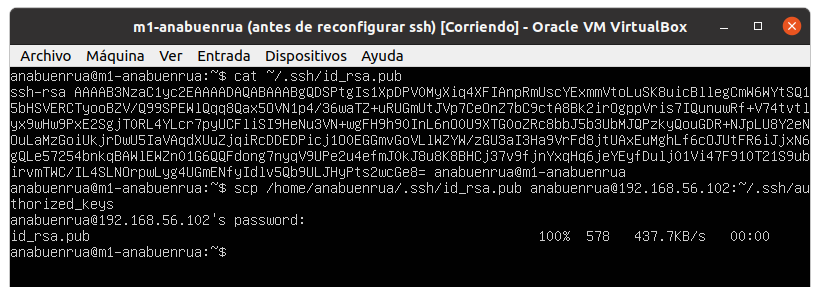
\includegraphics[scale=0.5]{ssh_6}
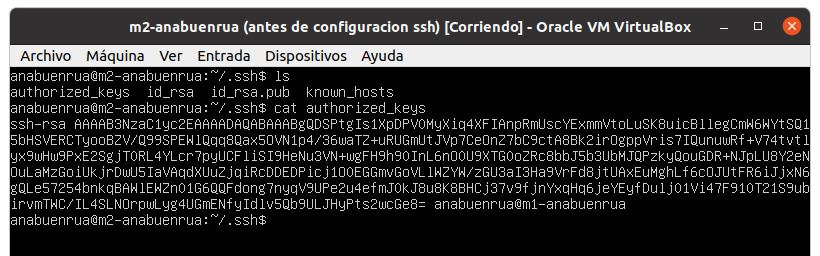
\includegraphics[scale=0.5]{ssh_7}
\end{center}
\end{figure}

Finalmente comprobamos que nos podemos conectar de m1 a m2 sin contraseña de nuevo conectándonos por ssh como en \eqref{ssh_8}.

\begin{figure}[h!]
\begin{center}
\caption{Conexión por ssh sin requerir introducir la contraseña.}
\label{ssh_8}
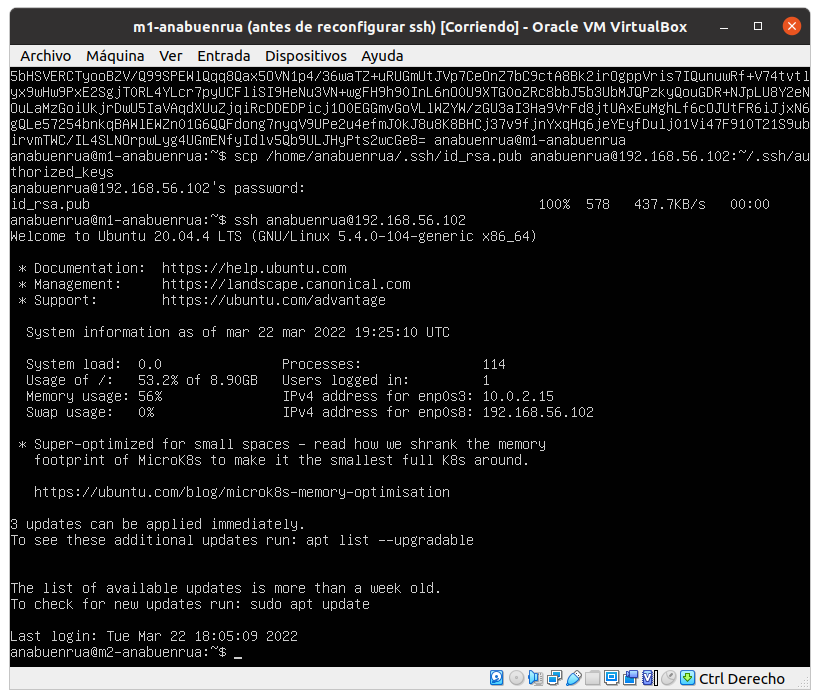
\includegraphics[scale=0.5]{ssh_8}
\end{center}
\end{figure}

\chapter{Usando crontab}

Comenzamos añadiendo una tarea que sincronice completamente las carpetas \verb|/var/www/| de m1 y de m2 cada hora.

Para conseguirlo, usamos crontab para programar la ejecución del comando de \verb|rsync| cada hora, editando el fichero \verb|/etc/crontab| como sigue en \eqref{crontab_1}.

\begin{figure}[h!]
\begin{center}
\caption{Configuración del fichero /etc/crontab para programar la sincronización con rsync cada hora.}
\label{crontab_1}
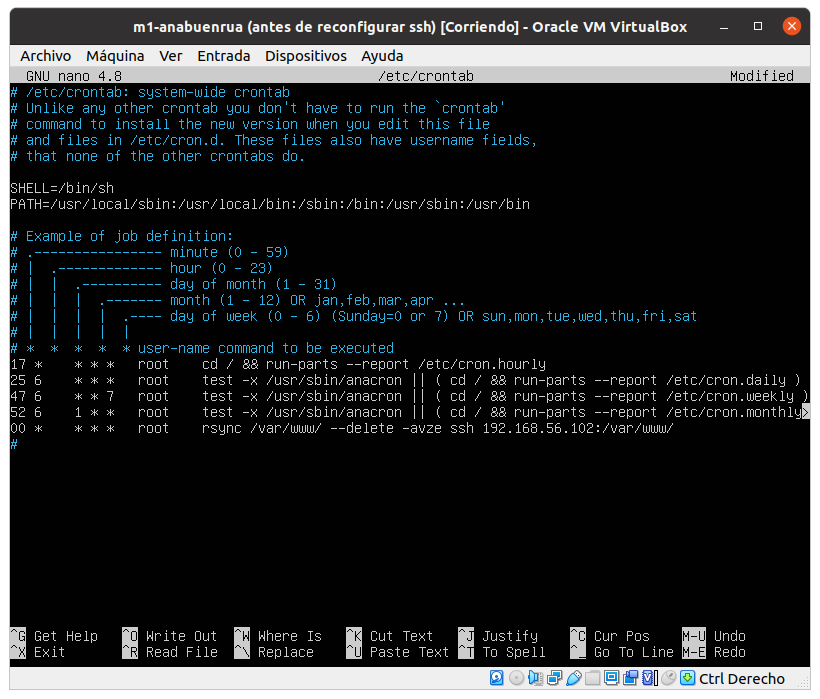
\includegraphics[scale=0.5]{crontab_1}
\end{center}
\end{figure}

\section{Opciones avanzadas}

Como opciones avanzadas, tenemos que mientras \verb|'*'| es para cualquier valor y se pueden especificar varios valores concretos separados por \verb|','|, hay formas más fáciles de especificar cuándo ejecutar ciertas tareas.

Por ejemplo, \verb|'-'| indica un rango, y \verb|'/'| el paso o salto. Así, si añadimos la siguiente tarea para escribir 'hola' en un fichero \verb|cronprueba.log| cada 2 horas los días 1,2 y 3 (de 1 a 3) sería editando el fichero \verb|/etc/crontab| como se ve en \eqref{crontab_2}

\begin{figure}[h!]
\begin{center}
\caption{Configuración del fichero /etc/crontab para escribir hola en un fichero los días 1,2 y 3 cada 2 horas.}
\label{crontab_2}
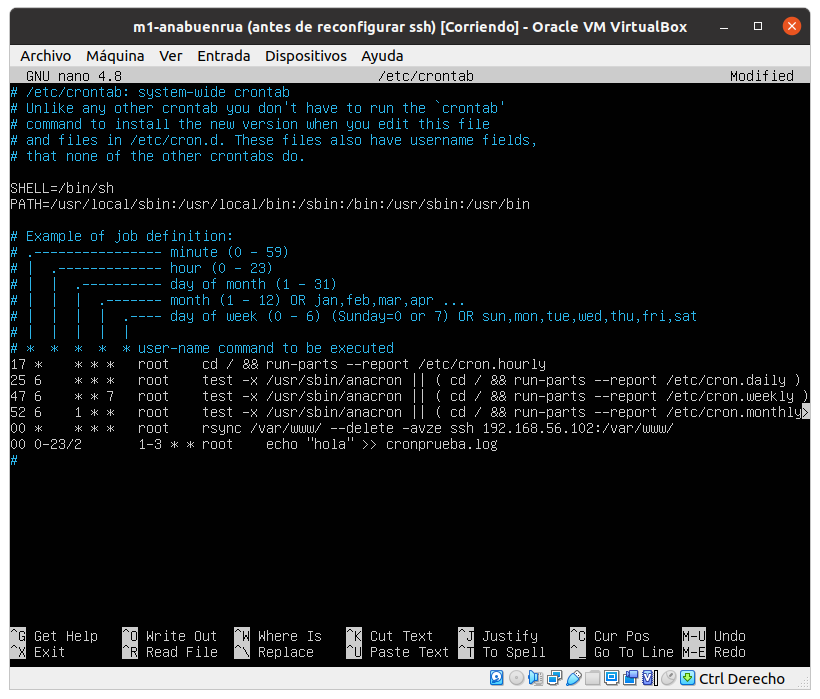
\includegraphics[scale=0.5]{crontab_2}
\end{center}
\end{figure}

\begin{verbatim}
00 0-23/2 1-3 * * root echo "hola" >> cronprueba.log
\end{verbatim}

Vemos que hemos especificado los minutos a 00 y en las de horas de 0 a 23 cada 2, en los días 1 a 3.










